\documentclass[12pt,letterpaper]{article}

\usepackage{lmodern}
\usepackage[T1]{fontenc}
%===========================
% disable section numbers
\renewcommand{\thesection}{}
\renewcommand{\thesubsection}{\arabic{section}.\arabic{subsection}}
\makeatletter
\def\@seccntformat#1{\csname #1ignore\expandafter\endcsname\csname the#1\endcsname\quad}
\let\sectionignore\@gobbletwo
\let\latex@numberline\numberline
\def\numberline#1{\if\relax#1\relax\else\latex@numberline{#1}\fi}
\makeatother
%===========================

\usepackage{amsmath} % math
\usepackage{shortvrb} % make "" behave like \texttt
\usepackage{hyperref} % hyper-referencing/link capabilities in PDF
\usepackage{xcolor} % colours for making hyperlinks look nicer
\hypersetup{
	colorlinks,
	linkcolor={red!50!black},
	citecolor={blue!50!black},
	urlcolor={blue!50!black}
}
\usepackage[margin=1in]{geometry} % control size of margins
%\usepackage{listings} % allow pretty formatting of stuff that needs pretty formatting
\usepackage{minted} % making nicely coloured code snippets
\usepackage[sorting=none]{biblatex} % bibliography
\usepackage{graphicx} % put in figures
\usepackage{siunitx} % pain-free angle representation in degrees (e.g. \ang{90}), other uses too

%=======================================

\newenvironment{custmint}[1]
{%
	\VerbatimEnvironment
	\begin{minted}{#1}%
	}
	{%
	\end{minted}%
}
\usepackage{mdframed} % for note boxes

\newmdenv[linewidth=2]{notebox} % note boxes

\MakeShortVerb" %see package shortvrb

% put something in quotation marks
\newcommand{\inquotes}[1]{``#1''}	% double quotes
\newcommand{\insquotes}[1]{`#1'}	% single quotes

% inline code short-hand
\newcommand{\ril}[1]{\mintinline[breaklines, breakanywhere]{rust}{#1}}
\newcommand{\cil}[1]{\mintinline[breaklines, breakanywhere]{c}{#1}}

\newcommand{\ash}{\texttt{ash}}

\newenvironment{indenttext}{%
	\par%
	\medskip
	\leftskip=4em\rightskip=2em%
	\noindent\ignorespaces}{%
	\par\medskip}

\let\oldquotation\quotation
\renewenvironment{quotation}{\begin{indenttext}\fontfamily{LinuxLibertineT-OsF}\selectfont}{\end{indenttext}}

%============ BIBLIOGRAPHY =============
\addbibresource{bibliography.bib}
%=======================================

\begin{document}

\title{Using Vulkan with Rust via \ash}
\date{0.1}
\author{Brian Merchant}
\maketitle
\tableofcontents
\reversemarginpar

% -----------------------------------------

\begin{abstract}
    This document provides a Rust-based introduction to using Vulkan to create graphics. \href{https://github.com/MaikKlein/ash}{\ash}, a Rust wrapper around the C Vulkan API, is used to build a series of small programs (\inquotes{samples}) which iterate upon one another towards a final goal of displaying a 3D cube.  
\end{abstract}

\section{Setup}
    Necessary: install \href{https://www.lunarg.com/vulkan-sdk/}{Vulkan SDK}.
    
    Optional: read history of Vulkan on Wikipedia.
	
\section{\inquotes{C-ish}}
	C-ish is this document's shorthand for C/C++. Since the Vulkan API is written in C, being faimilar with certain features of C-ish is useful. Additionally, many existing Vulkan tutorials use C++. 
    
    However, this document does not assume intimacy with C-ish: in fact, the author has only a passing familiarity. The following is a complete list of concepts that will be directly or indirectly referenced within the document:
		\begin{itemize}
            \item syntax and concept differences between C-ish pointers and Rust references
            
			\item C-ish \href{https://en.wikibooks.org/wiki/C_Programming/Arrays_and_strings}{array}s
            
            \item relationship between  \href{https://en.wikibooks.org/wiki/C_Programming/Pointers_and_arrays}{pointers} and \href{https://en.wikibooks.org/wiki/C_Programming/Pointers_and_arrays#Pointers_and_Arrays}{arrays} in C-ish; why will one sometimes see \cil{int*} given as the type for an array of \cil{int}s?
            
            \item C-ish \href{https://en.wikibooks.org/wiki/C_Programming/Advanced_data_types}{"struct"s and "enum"s}
            
            \item the keyword \href{https://en.wikibooks.org/wiki/C_Programming/Advanced_data_types}{\cil{typdef}}
			
            \item the keyword \cil{void}
            
            \item the keyword \cil{NULL}
            
			\item \href{https://en.wikibooks.org/wiki/C_Programming/Procedures_and_functions}{function} definition syntax; what is a \inquotes{function prototype}? 
			
			\item what a \href{https://en.wikipedia.org/wiki/Mask_(computing)}{bit mask} is, and \href{https://stackoverflow.com/questions/10493411/what-is-bit-masking}{how it's used}
            
            \item \item what does \texttt{"\textbackslash0"} do in a string? 
		\end{itemize}
   
\section{Motivation}

This tutorial assumes that the reader is somewhat interested in displaying computationally generated images on a physical screen: a task that is evidently easy to state. Attempting to execute this task however, will bear testament to the vast number of interconnected systems, developed over decades, which must be marshalled to create applications using electronic computing devices, of which the display of graphics is a relatively new and one might argue, relatively small part since for majority of the history of computational devices, graphical displays were rudimentary, if not inexistent. 

To display a graphical image on an electronic device, one must:
    \begin{enumerate}
        \item have some system (mathematics, \inquotes{geometry}) for describing images without ambiguity that requires human interpolation to decipher (i.e. without words)
        
        \item have some system (\inquotes{raster graphics}) for digitally representing image data
        
        \item have a computing device capable of \emph{efficiently} converting mathematical descriptions of images into digital representations; these tasks are very computationally intensive, since each point (pixel) of raster image must be specified, and the number of pixels in any interesting picture tend to be very large---this computational difficulty spawned a whole family of computing devices geared specifically towards performing many small calculations in parallel (\inquotes{graphics cards})
        
        \item have an electronic device \inquotes{CRT screen, LCD screen} capable of understanding/presenting digital image data: i.e. capable of converting image data into a physical format our eyes can interpret
    \end{enumerate}

The hardware (physical) software (digital, programmatic) systems required are less standardized than the mathematical systems involved. There is more than one vendor of Graphical Processing Units (GPUs), Central Processing Units (CPUs), screens, operating systems for managing these devices etc. and they are often engaged in economic competition, so standardization has been a slow, but steady process. Vulkan is the result of this process of standardization: it provides specification documents and software-side infrastructure to facilitate software-hardware communication by presenting a standardized interface joining software developers from one side with hardware developers on the other. 

People began to notice that there is no reason why one should \emph{only} perform graphics related computations in parallel on a graphics card, as there are many applications that can take advantage of the highly parallel nature of such physical devices. In fact, as Moore's prediction of exponentially increase processing speeds of electronic processors begins to tangle with engineering/physical limits, people are increasingly putting what were traditionally single processors into groups that work together. 

The marketing for Vulkan API is in many ways, is a product of this trend as it portrays Vulkan as not only a graphics API, but also a general \inquotes{compute} API. While it is true that compared to previous APIs such as OpenGL (highly specialized for graphics), Vulkan is designed with a far more abstract view of the computations it facilitates, the OpenCL API (developed by the same organization behind Vulkan) is \href{https://www.lunarg.com/faqs/vulkan-opencl-general-computing/}{a better choice} for handling general (usually scientific) highly-parallelized and/or heterogeneous system computations. Still, there is something to be said for Vulkan's abstracted organization, as it makes possible \href{https://www.lunarg.com/faqs/vulkan-opencl-interoperability/}{future convergence of OpenCL with Vulkan}.


\section{Introduction to Vulkan}

Vulkan provides an interface between software applications and a Vulkan-compatible physical devices. Vulkan compatible physical devices can be:
	\begin{itemize}
		\item a CPU
		\item \href{https://www.reddit.com/r/vulkan/comments/5f7jhn/is_it_possible_to_run_vulkan_on_cpu/}{a software abstraction running on top of a CPU}
		\item special purpose hardware for highly-parallel computing, e.g. a GPU;
		\item many CPUs configured to share data with each other
	\end{itemize}
A physical device is Vulkan compatible if somewhere, sometime, effort was put into writing a \inquotes{driver} meant to organize transfer of data between hardware and software as per the Vulkan specification. Thus, Vulkan standardizes communication between software and a wide variety of hardware.

Vulkan commands that form the interface between application and hardware drivers are brought into action by a \inquotes{loader}. Vulkan's specification calls for its core commands and the drivers they communicate with to be highly specialized for software-silicon crosstalk, so extraneous capabilities (such as debugging conveniences) are provided through optional (chosen by the programmer) \inquotes{layers} which are placed between the loader-driver conduit.    

Thus, to begin, a programmer creates an \inquotes{instance} of the loader. Through this loader instance, they search system for physical devices with Vulkan-compatible drivers. They choose specific physical devices to work with, and set which optional features of the physical devices should be used (e.g. use 64-bit floats, or 32-bit floats?). For each physical device, the programmer defines one or more \inquotes{logical devices}: abstractions representing subsets of a physical device's resources. Each logical device is used to create \inquotes{queues}, which are selected from several types of \inquotes{queue families}. Not all physical devices may implement every type of queue family, as different queue families are specialized for transferring particular types/formats of information. Finally, the programmer enables Vulkan API \inquotes{extensions} which provide convenient functions to handle specific tasks (e.g. graphics display).

From now on in this document, \inquotes{device} without qualification shall refer to a \inquotes{logical device} while a physical device will only be referred to in full as \inquotes{physical device}.

\begin{quotation}
    Vulkan exposes one or more devices, each of which exposes one or more queues which may process work asynchronously to one another. The set of queues supported by a device is partitioned into families. Each family supports one or more types of functionality and may contain multiple queues with similar characteristics. Queues within a single family are considered compatible with one another, and work produced for a family of queues can be executed on any queue within that family. This Specification defines four types of functionality that queues may support: graphics, compute, transfer, and sparse memory management.
\end{quotation}

\section{0: \texttt{init-instance.rs}}

A Vulkan \emph{instance} has C-ish type \cil{vkInstance}. One could create many \cil{vkInstance}s, if it is helpful for their task, but we only need to create one. In C-ish, an instance is created by calling the function \cil{vkCreateInstance}, which has the prototype:
		\begin{minted}{c}
VkResult vkCreateInstance(
const VkInstanceCreateInfo*                 pCreateInfo,
const VkAllocationCallbacks*                pAllocator,
VkInstance*                                 pInstance);
		\end{minted}
        
		\begin{itemize}
			\item return type \cil{vkResult}: a C-ish "enum", which contains a bunch of  constants indicating the result of different Vulkan commands: in this case, success (i.e. successful creation of an instance), or some sort of a failure
			
			\item argument \cil{pCreateInfo}: a pointer to a \cil{vkInstanceCreateInfo} "struct"
			
			\item argument \cil{pAllocator}: a pointer to a \cil{vkAllocationCallbacks} "struct" whose members contain various functions you might have written to help the physical device organize its memory usage---we will tend to go simple, and not provide anything, in which case the physical device will use its default memory management routines
			
			\item argument \cil{pInstance} an \inquotes{opaque pointer} to an instance (an opaque pointer is a C-ish concept which provides a pointer to a data structure, but the pointer cannot be used to query details of the data structure, nor can it be de-referenced)
		\end{itemize}

Let us examine the "struct" \cil{vkInstanceCreateInfo}, since we need to provide \cil{vkCreateInstance} with one:
		\begin{minted}{c}
typedef struct VkInstanceCreateInfo {
	VkStructureType             sType;
	const void*                 pNext;
	VkInstanceCreateFlags       flags;
	const VkApplicationInfo*    pApplicationInfo;
	uint32_t                    enabledLayerCount;
	const char* const*          ppEnabledLayerNames;
	uint32_t                    enabledExtensionCount;
	const char* const*          ppEnabledExtensionNames;
} VkInstanceCreateInfo;
		\end{minted}
		\begin{itemize}
			\item \cil{sType}: a member common to all Vulkan \inquotes{info "struct"}s, it indicates the type of the info "struct", in this case \cil{VK_STRUCTURE_TYPE_INSTANCE_CREATE_INFO}---this is useful because in C, you might sometimes get a typeless (\cil{void*}) pointer to a particular "struct", and to determine what kind of "struct" it is, you could query the \cil{sType} field
			
			\item \cil{pNext}: another common info "struct" member, usually set to \cil{NULL} unless API extensions (and only extensions) require one to pass additional "struct"s
			
			\item \cil{flags}: for future Vulkan versions, currently no flags defined, set to "0"
			
			\item \cil{pApplicationInfo}: pointer to a \cil{VkApplicationInfo} "struct" which we will study next
			
			\item \cil{ppEnabledLayerNames}: in this tutorial, we will not be using layers, so we can set this to \cil{NULL}
			
			\item \cil{enabledLayerCount}: length of the \cil{ppEnabledLayerNames} list thus should be zero since we have \cil{ppEnabledLayerNames == NULL}
			
			\item \cil{ppEnabledExtensionNames}: at this point in the tutorial, we are not using extensions, so we'll be setting this to \cil{NULL}
			
			\item \cil{enabledExtensionCount}: length of the \cil{ppEnabledExtensionNames} list
		\end{itemize}
This "struct" has which has some members typical to many other Vulkan info "struct"s, as the reader will see. \cil{vkInstanceCreateInfo} "struct" requires as a member an instance of the \cil{VkApplicationInfo} "struct" meant to provide some information regarding the application initializing the loader:
		\begin{minted}{c}
typedef struct VkApplicationInfo {
	VkStructureType    sType;
	const void*        pNext;
	const char*        pApplicationName;
	uint32_t           applicationVersion;
	const char*        pEngineName;
	uint32_t           engineVersion;
	uint32_t           apiVersion;
} VkApplicationInfo;
		\end{minted}
	\begin{itemize}
		\item \cil{sType}, \cil{pNext}: common features of many Vulkan info "struct"s, see the \cil{vkInstanceCreateInfo} "struct"'s member overview, as these are the same;
		
		\item \cil{pApplicationName}, \cil{applicationVersion}, \cil{pEngineName}, \cil{engineVersion}: for general use, e.g. sometimes drivers may be designed to execute special behaviour for certain application---this can be used to let them know which application they are dealing with
		
		\item \cil{apiVersion}:  this field communicates the major, minor, and patch levels of the Vulkan API used by the application; we'll be using "VK\_API\_VERSION\_1\_0" (major is "1", minor is "0").
	\end{itemize}

In "/init-instance/src/main.rs" we initialize a loader. Points to note and questions to consider:
	\begin{itemize}
		\item comments explaining \ril{use} statements
		
		\item \ril{unsafe} block: \ash an almost one-to-one interface to the Vulkan C API, thus many of Rust's safety features have to be disabled
		
		\item for fields like \cil{pApplicationName} we create a \ril{std::ffi::CString} and then pass it \inquotes{raw} (i.e. as a pointer) by calling \ril{as_ptr}, rather than using the standard Rust \ril{String}
		
		\item \ril{vk::StructureType} is used to fill out \ril{s_type} fields
		
		\item can you explain how the \ril{flags} field is filled out? (hint: look up the definition of the \ril{vk::InstanceCreateInfo} "struct" in \href{https://docs.rs/ash}{\ash's documentation} and then answer: what type is \ril{flags}? How is the \ril{std::Default} trait implemented for it?)
		
		\item that to actually use Vulkan, we first initialize an \ril{ash::Entry} "struct" which contains the supporting infrastructure to allow Rust to interface with Vulkan's C implementation
		
		\item the \ril{ash::Entry} "struct" also has some \ril{impl}s which put syntactic sugar around calling functions like \ril{vkCreateInstance}, in particular the function \ril{create_instance}---can you find where that function is implemented? (hint: open up \href{https://docs.rs/ash}{\ash's documentation}, and 1) figure out where the \ril{EntryV1_0} trait is defined, 2) figure out where \ril{Entry<V>} is defined, and 3) how is the \ril{EntryV1_0} implemented for \ril{Entry<V1_0>}?)
		
		\item we have to manually destroy the instance once we're done
	\end{itemize} 
	
To see everything in action: 
	\begin{center}
		"cargo run --bin init-instance"
	\end{center}
	
\section{1: \texttt{enumerate-devices.rs}}
	Obtaining a list of information from the loader is a common operation, and in the course of this tutorial, we will note that there is a pattern to how the API handles these operations. The pattern is well demonstrated by the next task: querying the loader for a list of available Vulkan-compatible physical devices on the host system. We call the function \cil{vkEnumeratePhysicalDevices}, which has prototype
	\begin{minted}{c}
VkResult vkEnumeratePhysicalDevices(
	VkInstance                                  instance,
	uint32_t*                                   pPhysicalDeviceCount,
	VkPhysicalDevice*                           pPhysicalDevices);
	\end{minted}
    
    The specification explains the function's arguments succinctly:
        \begin{quotation}
            If "pPhysicalDevices" is "NULL", then the number of physical devices available is returned in "pPhysicalDeviceCount". Otherwise, "pPhysicalDeviceCount" must point to a variable set by the user to the number of elements in the "pPhysicalDevices" array, and on return the variable is overwritten with the number of handles actually written to "pPhysicalDevices". If "pPhysicalDeviceCount" is less than the number of physical devices available, at most "pPhysicalDeviceCount" structures will be written. If "pPhysicalDeviceCount" is smaller than the number of physical devices available, "VK_INCOMPLETE" will be returned instead of "VK_SUCCESS", to indicate that not all the available physical devices were returned.
        \end{quotation}
    
    Assume we have a \cil{vkInstance} called \cil{instance} created, as explained in the last section, and a pointer to memory where we can store an unsigned integer \cil{pPhysicalDeviceCount}. Then, for our purposes, we would:
		\begin{enumerate}
            \item call \cil{vkEnumeratePhysicalDevices(instance, pPhysicalDeviceCount, NULL)} since we do not have a pre-existing array of devices, and are interested in finding out how many such devices exist; if \cil{vkResult} indicates success ("VK_SUCCESS" is returned), then \cil{pPhysicalDeviceCount} now points to an integer counting the number of physical devices available otherwise the specification states we get errors "VK_ERROR_OUT_OF_HOST_MEMORY", "VK_ERROR_OUT_OF_DEVICE_MEMORY", "VK_ERROR_INITIALIZATION_FAILED"
			
			\item assuming success, create an empty array of \cil{VkPhysicalDevice}s containing enough space for \cil{*pPhysicalDeviceCount} items "pPhysicalDevices" ("p" in the variable name stands for \inquotes{pointer})
			
			\item call \cil{vkEnumeratePhysicalDevices(instance, pPhysicalDeviceCount, pPhysicalDevices}---if \cil{vkResult} indicates success, then our list \cil{pPhysicalDevices} should be filled out with the \cil{vkPhysicalDevice}s
		\end{enumerate}
	
	In Rust-land, the \ril{ash::Instance} "struct" has an \ril{impl} function \ril{ash::Instance::enumerate_physical_devices}, which calls \cil{vkEnumeratePhysicalDevices} and returns a vector of \ril{vk::PhysicalDevice}s. The reader should look at the source code of this function:  \href{https://gist.github.com/bzm3r/175cd2b63db8f783ed968df20462be67}{gist link for annotated \ril{enumerate_physical_devices}}. To find the source, go to \ash's documentation for \ril{ash::Instance}, and click the appropriate "[src]" links. You can see that under the hood, \ash performs the operations we outlined above. 
	
	"enumerate-devices.rs" contains the code to enumerate physical devices on a system and print out how many were found. Note that before the program panics intentionally, care is taken to ensure that any instances we create are destroyed with the help of the \ril{unsafe} function \ril{destroy_instance_and_panic}. Run the program with the command: 
		\begin{center}
			"cargo run --bin enumerate-devices"
		\end{center}
    
	
\section{2: \texttt{init-device.rs}}

    The rest of this document assumes the at least one physical device exists on the host system. Creation of logical device abstractions over found physical devices will now be explored. Apart from organizing available physical resources, a logical device allows for the creation of queues which pass data between applications and physical devices. 
		
	For the sake of simplicity, let us select the first (perhaps only) physical device found. What queue families (types of queues) does it support? The list of available queue families can be obtained by calling \cil{vkGetPhysicalDeviceQueueFamilyProperties}, which has prototype:
		\begin{minted}{c}
void vkGetPhysicalDeviceQueueFamilyProperties(
	VkPhysicalDevice                            physicalDevice,
	uint32_t*                                   pQueueFamilyPropertyCount,
	VkQueueFamilyProperties*                    pQueueFamilyProperties);
		\end{minted}
	This function has the same organization as "vkEnumeratePhysicalDevices" seen in the previous section: after all, it too returns a list of data. Thus, similar to \ril{ash::Instance::enumerate_physical_devices}, \ash wraps the querying process in the "impl" function \ril{ash::Instance::get_physical_device_queue_family_properties}. Examining this function's source will reveal its similarities to \ril{ash::Instance::enumerate_physical_devices}. A successful call to \cil{get_physical_device_queue_family_properties} provides a list:  \ril{Vec<vk_sys::QueueFamilyProperties>}.
		
	What's inside C-ish \cil{vkQueueFamilyProperties}?
	   \begin{minted}{c}
typedef struct VkQueueFamilyProperties {
	VkQueueFlags    queueFlags;
	uint32_t        queueCount;
	uint32_t        timestampValidBits;
	VkExtent3D      minImageTransferGranularity;
} VkQueueFamilyProperties;

typedef enum VkQueueFlagBits {
	VK_QUEUE_GRAPHICS_BIT = 0x00000001,
	VK_QUEUE_COMPUTE_BIT = 0x00000002,
	VK_QUEUE_TRANSFER_BIT = 0x00000004,
	VK_QUEUE_SPARSE_BINDING_BIT = 0x00000008,
} VkQueueFlagBits;
	   \end{minted}
		\begin{itemize}
			\item \cil{queueCount}: unsigned integer specifying how many queues this device has 
			\item \cil{vkQueueFlags}: a bit mask of one or more \cil{VkQueueFlagBits} specifying the capabilities of queues in this family (some or all of Graphics, Compute, Transfer or Sparse).
		\end{itemize}
		
	\ash has a special type for these flag bits, \ril{ash::types::QueueFlags}, which also allow bitwise operations. Thus, we can convert the returned flag from hexadecimal to binary to determine the queue family's capabilities:
    	\begin{align*}
    		\mathtt{0x1} &\rightarrow 000\underline{1} && \text{Graphics}\\
    		\mathtt{0x2} &\rightarrow 00\underline{1}0 && \text{Compute}\\
    		\mathtt{0x3} &\rightarrow 0\underline{1}00 && \text{Transfer}\\
    		\mathtt{0x4} &\rightarrow \underline{1}000 && \text{Sparse}
    	\end{align*}
     For example, the flag "0xF" is $1111$ in binary, meaning that the queue family supports Graphics, Compute, Transfer, and Sparse operations, while flag "0x5", in binary is $0101$, meaning that only Graphics and Transfer operations are supported.
         
	To test whether a particular bit is set (i.e. is $1$), the \ril{subset} \ril{impl} for \ril{ash::types::QueueFlags} can be used, as demonstrated by  \ril{get_queue_family_supported_ops} in "init-device-0.rs". This program prints out queue families supported by the first physical device in the list of physical devices available on the host system.
		
\subsection{\texttt{init-device-and-queue.rs}}
	"init-device.rs" will now be iterated upon by by adding functionality to choose a physical device which has a queue family with graphics capability, since the tutorial ultimately aims to display a cube. One an appropriate physical device has been chosen, a \emph{logical device} is created on it, which will be used to create a queue from the graphics family. A broad outline for executing this procedure using the C-ish API is:
		\begin{enumerate}
			\item fill out a \cil{VkDeviceQueueCreateInfo} "struct" based on the queue family selected for each queue that will be created, and store each such "struct" in an array, perhaps called \cil{pQueueCreateInfos}
				
			\item fill out a \cil{VkDeviceCreateInfo} "struct", which amongst other members, requires \cil{pQueueCreateInfos}
                
			\item call \cil{vkCreateDevice}, which takes as an argument \cil{VkDeviceCreateInfo}, and will create \cil{vkDevice} upon success
				
			\item perform any tasks we need to with the resulting \cil{vkDevice}
				
			\item destroy the device
		\end{enumerate}
		
	Let us look at \cil{VkDeviceQueueCreateInfo}:
\begin{minted}{c}
typedef struct VkDeviceQueueCreateInfo {
	VkStructureType             sType;
	const void*                 pNext;
	VkDeviceQueueCreateFlags    flags;
	uint32_t                    queueFamilyIndex;
	uint32_t                    queueCount;
	const float*                pQueuePriorities;
} VkDeviceQueueCreateInfo;
\end{minted}
	\begin{itemize}
		\item \cil{flags}: for use by future Vulkan versions, set to 0 
			
		\item \cil{queueFamilyIndex}: index of the queue's queue family properties in the array \cil{vkQueueFamilyProperties}
			
		\item \cil{queueCount}: the number of queues to be created (shouldn't be greater than the number of queues supported by the physical device, as specified in the queue family's properties!)
			
		\item \cil{pQueuePriorities}: an array of \cil{queueCount} normalized floating point values (i.e. "float"s between 0.0 and 1.0), denoting the relative priority of each queue we're creating: 0.0 is lowest priority, 1.0 is highest; within the physical device, queues with higher priority will have a higher chance of being allotted more processing time than queues with lower priority; more on this later
	\end{itemize}
		
	The "struct" \cil{VkDeviceCreateInfo} is defined like:
    \begin{minted}{c}
typedef struct VkDeviceCreateInfo {
    VkStructureType                    sType;
    const void*                        pNext;
    VkDeviceCreateFlags                flags;
    uint32_t                           queueCreateInfoCount;
    const VkDeviceQueueCreateInfo*     pQueueCreateInfos;
    uint32_t                           enabledLayerCount;
    const char* const*                 ppEnabledLayerNames;
    uint32_t                           enabledExtensionCount;
    const char* const*                 ppEnabledExtensionNames;
    const VkPhysicalDeviceFeatures*    pEnabledFeatures;
    } VkDeviceCreateInfo;
\end{minted}
	\begin{itemize}
		\item \cil{queueCreateInfoCount}: how many queue groups are to be associated with this logical device (each group will have its own \cil{vkDeviceQueueCreateInfo} "struct")
			
		\item \cil{pQueueCreateInfos}: list of \cil{vkDeviceQueueCreateInfo} "struct"s (count given by \cil{queueCreateInfoCount})
			
		\item \cil{enabledLayerCount} and \cil{ppEnabledLayerNames}: deprecated and ignored
			
   		\item \cil{enabledExtensionCount} and \cil{ppEnabledExtensionNames}: to be discussed later in the document, for now \cil{0} and \cil{NULL} respectively
   		
   		\item \cil{pEnabledFeatures}: to be discussed later in the document, for now \cil{NULL}
   	\end{itemize}
	
    Hints of more advanced features available, such as Vulkan API extensions or optional physical device features are beginning to appear, but we ignore these for the time being.
		
	The analogues of \cil{VkDeviceQueueCreateInfo} and \cil{VkDeviceCreateInfo} in \ash are \ril{vk::DeviceQueueCreateInfo} (\href{https://docs.rs/ash/0.20.2/ash/vk/types/struct.DeviceQueueCreateInfo.html}{docs}) and \ril{vk::DeviceCreateInfo} (\href{https://docs.rs/ash/0.20.2/ash/vk/types/struct.DeviceCreateInfo.html}{docs}) respectively. "init-device-1.rs" selects a physical device graphics capable queue families, fills out \ril{vk::DeviceQueueCreateInfo} and \ril{vk::DeviceCreateInfo}, and then calls \ril{ash::Instance::create_device}. Before exiting, it cleans up by destroying the created device, and the underlying loader instance. This example only creates one queue, but if more were to be created, we would provide a Rust array or vector of \ril{vk::DeviceQueueCreateInfo} in raw pointer form through \ril{.as_ptr}. This provides a C-ish style list of objects, which can be accessed through offsetting of the pointer.
		
	Study the code in "init-device-and-queue.rs" and then run it:
    	\begin{center}
    		"cargo run --bin init-device-and-queue"
    	\end{center}
      
\section{3: \texttt{init-command-buffer.rs}}
	In the Vulkan model of execution, an application records commands into a buffer, which is passed to physical device drivers Since instructions are received in batches, drivers are able to use knowledge of upcoming instructions to optimize execution of the entire batch. 
    
	Since aive implementations for creating and destroying individual command buffers can be very inefficient, Vulkan provides \inquotes{command buffer pools}, which manage the creation and destruction of command buffers using \inquotes{pool allocators}. Another source of inefficiency can be the processing of many command buffers, each with a small number of instructions, so pools also provide solutions here. Since pools are allocated based on the type of queue family their commands are intended for, every command buffer pool is associated with a single queue family available to the physical device.
	
	To create a command buffer pool, a \cil{vkCommandPoolCreateInfo} "struct" is submitted to the \cil{vkCreateCommandPool} function:
	\begin{minted}{c}
typedef struct VkCommandPoolCreateInfo {
	VkStructureType             sType;
	const void*                 pNext;
	VkCommandPoolCreateFlags    flags;
	uint32_t                    queueFamilyIndex;
	} VkCommandPoolCreateInfo;

VkResult vkCreateCommandPool(
    VkDevice                                    device,
    const VkCommandPoolCreateInfo*              pCreateInfo,
    const VkAllocationCallbacks*                pAllocator,
    VkCommandPool*                              pCommandPool)
	\end{minted}
		\begin{itemize}
			\item \cil{sType}: set to \cil{VK_STRUCTURE_TYPE_COMMAND_POOL_CREATE_INFO}
			
			\item \cil{pNext}: typical info "struct" member
			
			\item \cil{flags}: a bitmask of \cil{VkCommandPoolCreateFlagBits} indicating pool usage and behaviour attributes. Possible bits are:
				\begin{itemize}
					\item \cil{VK_COMMAND_POOL_CREATE_TRANSIENT_BIT} (0x1): command buffers allocated from the pool will be short-lived
					
					\item \cil{VK_COMMAND_POOL_CREATE_RESET_COMMAND_BUFFER_BIT} (0x2): when a command buffer is first allocated is in the initial state, and command pools with the reset bit set allow buffers from the pool to be reset to their initial state
				\end{itemize}
			
			\item \cil{queueFamilyIndex}: index of the queue family that the command pool will be associated with 
            
			\item \cil{device}: logical device which will manage creating the command pool
			
			\item \cil{pCreateInfo}: a pointer to a filled out \cil{vkCreateCommandPool} "struct"
			
			\item \cil{pAllocator}: standard input described in earlier sections
			
			\item \cil{pCommandPool}: a pointer to a \cil{vkCommandPool}, which \cil{vkCreateCommandPool} will associate with the newly created pool
		\end{itemize}
    
	Once a command pool is created, it is stored in a \cil{VkCommandBufferAllocateInfo} "struct", which is submitted to a call of \cil{vkAllocateCommandBuffers}:
		\begin{minted}{c}
typedef struct VkCommandBufferAllocateInfo {
	VkStructureType         sType;
	const void*             pNext;
	VkCommandPool           commandPool;
	VkCommandBufferLevel    level;
	uint32_t                commandBufferCount;
	} VkCommandBufferAllocateInfo;
    
VkResult vkAllocateCommandBuffers(
    VkDevice                                    device,
    const VkCommandBufferAllocateInfo*          pAllocateInfo,
    VkCommandBuffer*                            pCommandBuffers);
		\end{minted}
        
		\begin{itemize}
			\item \cil{sType}: set to \cil{VK_STRUCTURE_TYPE_COMMAND_BUFFER_ALLOCATE_INFO}
			
			\item \cil{pNext}: standard info "struct" member
			
			\item \cil{commandPool}: command pool that was created
			
			\item \cil{level}: the "enum" \cil{VkCommandBufferLevel} has values \cil{VK_COMMAND_BUFFER_LEVEL_PRIMARY} and \cil{VK_COMMAND_BUFFER_LEVEL_SECONDARY}, which specify whether this command buffer is primary or secondary---a primary command buffer can be submitted to a queue, while a secondary command buffer cannot be submitted to a queue, but can be executed by a primary command buffer; primary command buffers cannot be executed by secondary ones
			
			\item \cil{commandBufferCount}: how many buffers to make with these settings

			\item \cil{vkDevice}: the device with which the command pool is associated
			
			\item \cil{pAllocateInfo}: pointer to a filled out \cil{VkCommandBufferAllocateInfo} struct
			
			\item \cil{VkCommandBuffer}: a pointer to an array of \cil{VkCommandBuffer}s where the newly created command buffers will be stored (so, the array should have length at least \cil{commandBufferCount} set in the \cil{VkCommandBufferAllocateInfo} "struct")
		\end{itemize}
	
	Using Rust, assuming a logical device has been created:
		\begin{enumerate}
            \item use logical device's \ril{impl} \ril{create_command_pool} for creating a command pool
            
			\item store info used to create a command pool in a \ril{vk::CommandPoolCreateInfo} "struct"
			
			\item store info used to allocate command buffers in a \ril{vk::CommandBufferAllocateInfo} "struct"
			
			\item use logical device's \ril{impl} \ril{allocate_command_buffers} for allocating buffers
			
			\item use command pool as necessary
			
			\item destroy command pool with logical device's \ril{impl} \ril{destroy_command_pool}
		\end{enumerate}
    
	These steps are implemented in "init-command-buffer.rs". Note that our clean ups are becoming more complicated, necessitating a new function \ril{clean_up}, which can handle clean up of instances, devices, and pools. 
	
	In the last sample of this tutorial series, we will record commands to command buffers, and submit them to a physical device using Vulkan-provided \cil{vkQueueSubmit}'s Rust analogue. Between now and then, necessary preparatory steps are undertaken.

\section{The Graphics Pipeline}
    In the coming sections, we will familiarize ourselves with Vulkan extensions that are gearted towards real time computer graphics applications. Since the Vulkan specification often makes references to concepts related to this process, having an understanding of how it works will be helpful.

    The creation (\inquotes{rendering}) of 3D images using a computer can be broadly separated into categories:
        \begin{enumerate}
            \item ahead-of-time rendering: these rendering processes are well suited towards creating 3D images which require time-intensive computations (e.g. for lighting, see: https://en.wikipedia.org/wiki/Ray_tracing_(graphics)) to render highly realistic scenes, detailed animations, or other advanced effects; used for movies, game cut scenes, 3D art, etc.
            
            \item on-demand rendering: these rendering processes are well suited towards creating 3D images for interactive applications, such as games or user interfaces, which require something like at least 25 frames per second to produce the illusion of smooth animation; clever techniques are used to minimize rendering cost (for example, reflections on glossy surfaces, but instead the scene from the perspective of the surface would be painted on as an approximation), at the cost of losing realistic detail, or other advanced features
        \end{enumerate}

    
    The graphics pipeline is a conceptual organization of computing resources to handle the second case of on-demand rendering. APIs like Vulkan and its extensions are designed along the concepts of the graphics pipeline, which represent a series of computations (perhaps with loops?) data is passed through, with the end product being an image which can be displayed to the user. Vulkan allows the user to build and order the operations within the pipeline as required. The ordering of operations within a pipeline is referred to as "synchronization". We now look at an example of a typical Vulkan pipeline.
    
    \begin{figure}
        \centering
        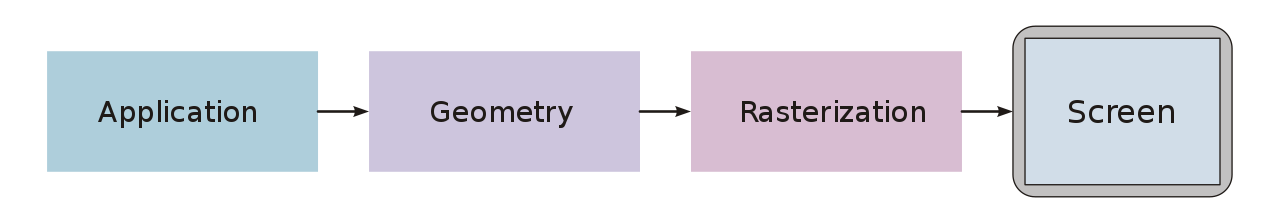
\includegraphics[width=0.7\linewidth]{Graphics_pipeline_2_en.svg}
        \caption{A diagram of a graphics pipeline showing only its most fundamental components. By \href{https://commons.wikimedia.org/wiki/File:Graphics_pipeline_2_en.svg}{PaterMcFly / Vierge Marie}.}
        \label{fig:graphicspipeline2en}
    \end{figure}
    
    \begin{figure}
        \centering
        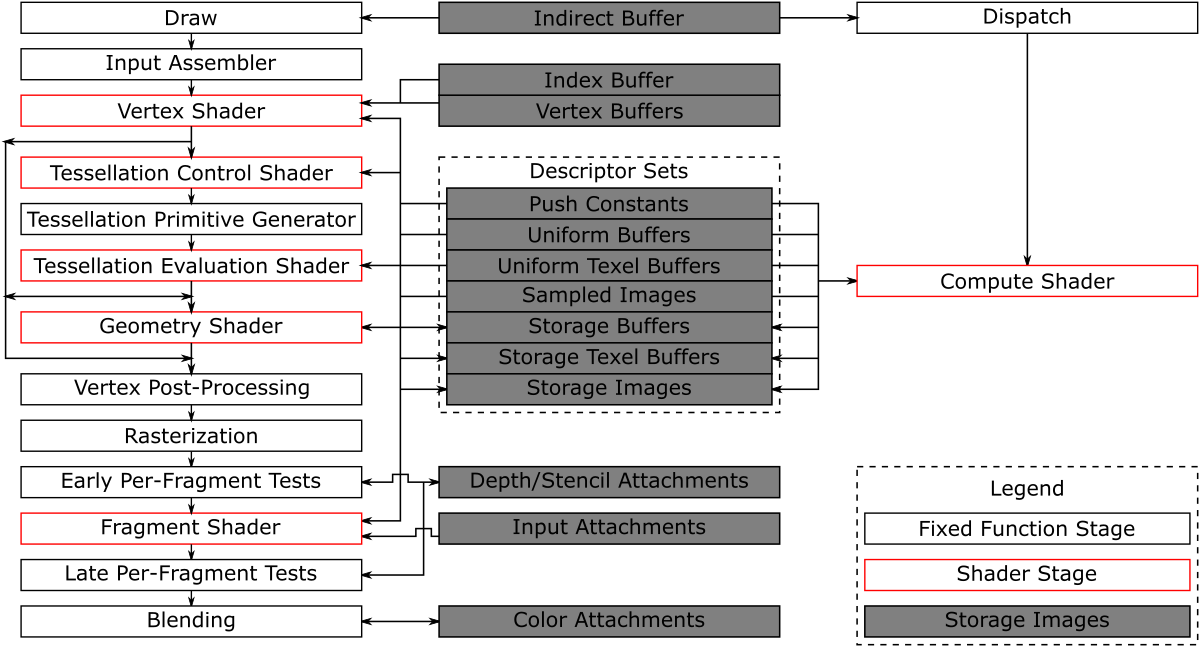
\includegraphics[width=0.7\linewidth]{vulkan-graphics-pipeline}
        \caption{A Vulkan graphics pipeline, showing all the different components that could be utilized. From the Vulkan specification.}
        \label{fig:vulkan-graphics-pipeline}
    \end{figure}
    
    The application provides computations that are run external to the pipeline. It selects which scenes need to be rendered, takes into account user input, collisions between physical object models, networking, and so on; in other words, it runs all the computations needed to provide the program of interest as a whole, and delegates graphics rendering to the graphics pipeline---when using Vulkan, the application does so by issuing drawing commands. This quote from the Vulkan specification shows how objects we have seen such as queues and command buffers come together to deliver drawing commands: 
        \begin{quotation}
            Drawing commands (commands with Draw in the name) provoke work in a graphics pipeline. Drawing commands are recorded into a command buffer and when executed by a queue, will produce work which executes according to the bound graphics pipeline. A graphics pipeline must be bound to a command buffer before any drawing commands are recorded in that command buffer.
        \end{quotation}
    After the application has issued graphics instructions using draw commands, these commands are transferred to the \inquotes{Input Assembler}, which puts together triangles, lines and points (geometric primitives) based on the requested commands. 

    Once these primitives have been generated, they are passed onto the Vertex Shader, which every Vulkan graphics pipeline must contain. The \inquotes{Vertex Shader} (\inquotes{shader} is simply jargon for a program for executing highly parallelizable tasks: for example, executing some instruction on a large number of vertices as input) computes the positions of the points and vertices assembled by the Input Assembler; one can think of the Input Assembler as defining the relationships between the various geometric primitives, based on drawing commands, but these primitives are not yet placed concretely in space, as this will depend upon the viewing angle, the zoom level, and so on. Having generated vertex data using the Vertex Shader, one can choose to pass this data through optional \inquotes{Tesselation} and \inquotes{Geometry} Shaders, which can do things like create more advanced shapes programmatically from primitives. 

    The vertex data is then passed through the Vertex Post-Processing step, where vertices which will not fit into the viewing area (see \href{https://en.wikipedia.org/wiki/Viewing_frustum}{related Wikipedia article}) are \inquotes{clipped}: that is, they will be essentially removed, since they will not be viewed within the scene. This way, computationally intensive operations do not need to be run on objects which will not be viewed in the first place. The clipped vertex data is then passed to the \inquotes{Rasterization} stage. 

    Rasterization refers to the process of converting a mathematical data representing an image (as we have at this stage of the pipeline, where our scene is made of primitives defined by their coordinates) into a 2D pixel image representation. Pixels are stored in memory using \inquotes{framebuffers} (\inquotes{frame} for an image frame, and \inquotes{buffer} for storage memory). The data Rasterization produces for a given pixel (its $(x, y)$ coordinates, address within the framebuffer, colour, depth, etc.) is called a "fragment" (see \href{https://en.wikipedia.org/wiki/Fragment_(computer_graphics)}{related Wikipedia article}). The next steps in the pipeline perform calculations which may modify the fragment. For instance, in the Early Per-Fragment tests stage, a technique called z-buffering (see \href{https://en.wikipedia.org/wiki/Z-buffering}{related Wikipedia article}) is used to figure out how objects in the scene occlude each other, depending on their \inquotes{depth} within the scene. This technique requires some additional memory per pixel, called the \inquotes{depth/stencil attachment} to keep track of the depth of various objects. Essentially, an attachment is a piece of memory, capable of being addressed in a per-pixel manner, that shaders can refer to (and even modify) as necessary. So, additional shaders and tests can be conducted, to perform a variety of operations needed to determine what data each fragment should finally contain (see the \href{https://en.wikipedia.org/wiki/Fragment_(computer_graphics)}{Wikipedia article on Fragments} for more examples of such operations). 

    There is some general vocabulary to talk about this stage of rendering, where each fragment is being updated based on the colours attached to objects, lighting, depth, and so on. A \inquotes{subpass} is a phase of rendering that reads and writes into certain attachments. Rendering commands, provided by the user are recorded in association with a particular subpass. Subpasses make up a \inquotes{render pass}, which is a collection attachments, subpasses, and \inquotes{subpass descriptions}. A subpass description describes which attachments are associated with a subpass (and whether they are read/write). 

    Some common type of attachments that are referred to in the specification are:
        \begin{itemize}
            \item color attachments: these include color information (perhaps also including how these colours should be blended) regarding various scene objects
            
            \item depth/stencil attachments: these are typically used for z-buffering (recall the Wikipedia article on this technique), and may be more specially called "depth attachments" in that case; otherwise, "stencil attachments" could refer to stenciling, which is a simple way of defining what parts of the screen are finally visible to the user (conceptually: if for example, if one wants to model looking through the keyhole of a door, one could "apply" a keyhole shaped stencil, which would block rendering of all pixels that are not within the keyhole)
            
            \item resolve attachments: useful in more advanced techniques, they store output data from programs (shaders?) which take into account multiple input attachments, or take into account how the data in a fragment might be influenced by its neighbours
        \end{itemize}
    
    Once a framebuffer is filled out with the finalized data in each fragment, it can be displayed to the user. Assuming the application is running on a personal computer, this would be done with the help of the PC's OS and accompanying \inquotes{window system}. However, the core Vulkan API doesn't assume this is a universal intention, so functionality relevant to this end is packaged separately in a Khronos (i.e. \inquotes{Official}) extensions, such as: "Swapchain", "Surface", "Win32Surface" or "XlibSurface". 

    The Vulkan specification defines \inquotes{presentation engine} as:
        \begin{quotation}
            The presentation engine is an abstraction for the platform’s compositor or display engine.
        \end{quotation}
    Vulkan provides an API for interaction with the presentation engine, which is an abstraction for all the pieces of hardware and software which take in graphics information, and then display it. 

    Importantly, the presentation owns \inquotes{presentable images}. One can think of these as blank slates which the application borrows from the presentation engine in order to fill it with relevant information (e.g. some graphics) (from framebuffers?). Once the application has filled in the presentable image, it returns it to the presentation engine, which will manage the display of the image. In particular, the presentation image doesn't simply paint the image onto a display as soon as the application hands it back, but rather, buffers presentable images through an abstraction called the \inquotes{swap chain}. In some sense, swap chains are an abstraction that facilitate the illusion of real-time, as Wikipedia explains:
        \begin{quotation}
            In computer graphics, a swap chain is a series of virtual framebuffers utilized by the graphics card and graphics API for frame rate stabilization and several other functions. The swap chain usually exists in graphics memory, but it can exist in system memory as well. The non-utilization of a swap chain may result in stuttering rendering, but its existence and utilization are required by many graphics APIs...In every swap chain there are at least two buffers. The first framebuffer, the screenbuffer, is the buffer that is rendered to the output of the video card. The remaining buffers are known as backbuffers. Each time a new frame is displayed, the first backbuffer in the swap chain takes the place of the screenbuffer, this is called "presentation" or swapping...
        \end{quotation}
    The Vulkan specification writes:
        \begin{quotation}
            A swap chain is an abstraction for an array of presentable images that are associated with a surface. The presentable images are represented by `VkImage` objects created by the platform. One image (which can be an array image for multiview/stereoscopic-3D surfaces) is displayed at a time, but multiple images can be queued for presentation. An application renders to the image, and then queues the image for presentation to the surface.
        \end{quotation}

    The presentation engine is exposed via Vulkan through its relevant extensions. The key components of the presentation engine are:
        \begin{itemize}
            \item windowing system integration (WSI): a process responsible for organizing the display of data emitted by a phsyical device. A "platform" is an abstraction for a window system (e.g. X Window System, MS Windows, Mir, Wayland, Android), an OS, or some combination of the above (e.g. MS Windows, Wayland, Android)---basically, whatever the \inquotes{platform} needs to display graphics data. Not all physical devices will have WSI support, and not all queue families on a physical device might support \inquotes{presentation} of images to a specified surface. Thus, the application will need to find a suitable physical device, and relevant queue families on it which support a specified surface.
            
            \item \inquotes{surface}: an abstraction of a display surface. In particular, the surface abstracts away a lot of the platform specific details of what windowing systems may call a \inquotes{window}.
            
            \item \inquotes{swap chain}: abstraction providing buffering of presentable images. 
        \end{itemize}

    We will now learn how to initialize a swap chain.

    
\section{4: \texttt{init-swap-chain.rs}}

    Recall the info "struct" we had to fill out in order to create a logical device:
\begin{minted}{c}
typedef struct VkDeviceCreateInfo {
	VkStructureType                    sType;
	const void*                        pNext;
	VkDeviceCreateFlags                flags;
	uint32_t                           queueCreateInfoCount;
	const VkDeviceQueueCreateInfo*     pQueueCreateInfos;
	uint32_t                           enabledLayerCount;
	const char* const*                 ppEnabledLayerNames;
	uint32_t                           enabledExtensionCount;
	const char* const*                 ppEnabledExtensionNames;
	const VkPhysicalDeviceFeatures*    pEnabledFeatures;
} VkDeviceCreateInfo;
\end{minted}

	Previously, \cil{enabledExtensionCount} and \cil{ppEnabledExtensionNames} were ignored, but now we will specify extension \texttt{"VK\_KHR\_swap chain"} as enabled. The following steps are necessary, using \ash:
		\begin{enumerate}
			\item \ril{use ash::extensions::swap chain} loads the module which contains swap chain extension related stuff
				
			\item create an array with the string \texttt{"VK\_KHR\_swap chain"} by using the \ril{name} static \ril{impl} of \ril{swap chain} (track down the source for \ril{ash::extensions::swap chain::name} as an exercise): 
\begin{minted}{rust}
let device_extension_names_pointers = [swap chain::name().as_ptr()];
\end{minted}
			
			\item set the \ril{enabled_extension_count} and \ril{pp_enabled_extension_names} members of the \ril{vk::DeviceCreateInfo} "struct" we fill out using \ril{device_extension_names_pointers.len() as u32} and \ril{device_extension_names_pointers} respectively
		\end{enumerate}
	
	Now, the \ril{device} created in "init-swap-chain.rs" will have the swap chain extension enabled. Note that all the work was essentially done by the platform dependent conditionally compiled function \ril{get_extension_names}. 
	
    We eventually want to create a surface, but a surface needs a \inquotes{window} associated with it. In Rust as in C-ish, there are various windowing libraries, but this tutorial uses \ril{extern crate winit}. This document will not discuss in depth the internals of a window system, which depend heavily upon the particular platform the application is running on. These details are explained in documentation for the \ril{winit} crate, amongst other sources.
    
    The following code in "init-swap-chain.rs", within the function \ril{create_events_loop_and_window} creates an event loop and a window:
    \begin{minted}{rust}
let events_loop = winit::EventsLoop::new();

let window = winit::WindowBuilder::new()
    .with_title("Ash - Example")
    .with_dimensions(window_width, window_height)
    .build(&events_loop)
    .unwrap();
    \end{minted}
    
    The event loop handles messages sent between the user interface (the window), and our application (e.g. user input). Further details are presented in \href{https://docs.rs/winit/0.10.0/winit/struct.EventsLoop.html}{the documentation} for \ril{winit::EventsLoop}. A window is created using self-explantory calls setting the title, dimensions and event loop. Given the \ril{window} from a windowing system, we create an associated surface using a platform dependent conditionally compiled function \ril{create_surface}, which is defined within "init-swap-chain.rs".
    
    We now have a surface, but we have not yet found a physical device on which we can create logical devices. Previously, we found a physical device supporting graphics on our system. However, just like in the case of graphics, not all physical devices support presentation so this time we must find a physical device which supports both graphics and presentation. Essentially, a physical device supports graphics and presentation if it has queue families capable of supporting graphics and presentation operations. Some queue families may support both, but this is not always the case, so we will also need to determine which queue families on the physical device are of interest to us. All of this logic is handled in the function \ril{find_pdevice_with_queue_family_supporting_graphics_and_presentation}. Note that in order to call this function, we need to pass a reference to an instance of a surface extension loader provided through the \cil{Surface} Khronos extension. This extension allows us to do things like check if a physical device supports presentation to a specified surface; essentially, it contains all sorts of utilities for dealing with surfaces. To use the capabilities of the extension, we load in an instance of its loader, which handles our requests for various utilities. In particular, if we were using C-ish, we would query for a queue's presentation support relative to a surface using the function:
    \begin{minted}{c}
VkResult vkGetPhysicalDeviceSurfaceSupportKHR(
    VkPhysicalDevice                            physicalDevice,
    uint32_t                                    queueFamilyIndex,
    VkSurfaceKHR                                surface,
    VkBool32*                                   pSupported);
    \end{minted}
    \begin{itemize}
        \item \cil{VkPhysicalDevice}: the physical device containing the queue
        
        \item \cil{queueFamilyIndex}: index of some queue family offered by the physical device
        
        \item \cil{surface}: the surface we created
        
        \item \cil{pSupported}: a pointer to "bool32" sized memory; "vkGetPhysicalDeviceSurfaceSupportKHR" will set its value depending on whether the queue family supports presentation to the surface (True for supported, False for not supported)
    \end{itemize}
    In Rust-land, Ash's wrapper around the \ril{Surface} extension allows us to call the function `get_physical_device_surface_support_khr` through an instance of the surface extension loader.
    
    Having determined which physical device is of interest, and which queue families on it are relevant, we can now create logical device and set up queues on it, and then we can set up command buffers and pools managing those queues. 
    
	In C-ish, to create a swapchain, one would begin by setting up "struct" \cil{VkSwapchainCreateInfoKHR}. We will explore the fields of this "struct" in detail later, and for now we learn how to query the physical device for information about the surface we have associated with it, so that we can use this information to fill in \cil{VkSwapchainCreateInfoKHR} later. To query the physical device, we use the function:
        \begin{minted}{c}
VkResult vkGetPhysicalDeviceSurfaceCapabilitiesKHR(
        VkPhysicalDevice                            physicalDevice,
        VkSurfaceKHR                                surface,
        VkSurfaceCapabilitiesKHR*                   pSurfaceCapabilities);
        \end{minted}
        
    This function fills out the following \cil{struct}:
        \begin{minted}{c}
typedef struct VkSurfaceCapabilitiesKHR {
    uint32_t                         minImageCount;
    uint32_t                         maxImageCount;
    VkExtent2D                       currentExtent;
    VkExtent2D                       minImageExtent;
    VkExtent2D                       maxImageExtent;
    uint32_t                         maxImageArrayLayers;
    VkSurfaceTransformFlagsKHR       supportedTransforms;
    VkSurfaceTransformFlagBitsKHR    currentTransform;
    VkCompositeAlphaFlagsKHR         supportedCompositeAlpha;
    VkImageUsageFlags                supportedUsageFlags;
} VkSurfaceCapabilitiesKHR;
        \end{minted}
    \begin{itemize}
        \item \cil{minImageCount}: minimum number of images physical device supports for a swap chain interfacing with surface (will be at least one)
        
        \item \cil{maxImageCount}: maximum number of images physical device supports for a swap chain interfacing with surface (will be either 0, meaning that there is no upper limit (apart from memory) or greater than or equal to \cil{minImageCount}) 
        
        \item \cil{currentExtent}: current width and height of the surface, or special value ($0xFFFFFFFF$, $0xFFFFFFFF$) indicating that surface size is governed by the extent of a swap chain interfacing with it
        
        \item \cil{minImageExtent}: smallest valid swap chain extent for surface---width and height of the extent will be less than or equal to width and height of \cil{currentExtent} (unless \cil{currentExtent} is the special value)
        
        \item \cil{maxImageExtent}: largest valid swap chain extent for surface---width and height given by \cil{maxImageExtent} will be greater than or equal to width and height of \cil{minImageExtent} and greater than or equal to width and height of \cil{currentExtent} (unless \cil{currentExtent} is the special value)
        
        \item \cil{maxImageArrayLayers}: maximum number of layers presentable images can have for a swap chain created for this device and surface, and will be at least one---\inquotes{image layers} are views in a multiview/stereo surface for stereoscopic-3D applications
        
        \item \cil{supportedTransforms}: bitmask of \cil{VkSurfaceTransformFlagBitsKHR} indicating presentation transforms supported for the surface (at least one bit will be set); \cil{VkSurfaceTransformFlagBitsKHR} is an \cil{enum}:
            \begin{minted}{c}
typedef enum VkSurfaceTransformFlagBitsKHR {
    VK_SURFACE_TRANSFORM_IDENTITY_BIT_KHR = 0x00000001,
    VK_SURFACE_TRANSFORM_ROTATE_90_BIT_KHR = 0x00000002,
    VK_SURFACE_TRANSFORM_ROTATE_180_BIT_KHR = 0x00000004,
    VK_SURFACE_TRANSFORM_ROTATE_270_BIT_KHR = 0x00000008,
    VK_SURFACE_TRANSFORM_HORIZONTAL_MIRROR_BIT_KHR = 0x00000010,
    VK_SURFACE_TRANSFORM_HORIZONTAL_MIRROR_ROTATE_90_BIT_KHR = 0x00000020,
    VK_SURFACE_TRANSFORM_HORIZONTAL_MIRROR_ROTATE_180_BIT_KHR = 0x00000040,
    VK_SURFACE_TRANSFORM_HORIZONTAL_MIRROR_ROTATE_270_BIT_KHR = 0x00000080,
    VK_SURFACE_TRANSFORM_INHERIT_BIT_KHR = 0x00000100,
} VkSurfaceTransformFlagBitsKHR;
            \end{minted}
            
            \begin{itemize}
                \item \cil{VK_SURFACE_TRANSFORM_IDENTITY_BIT_KHR}: specifies that the \inquotes{identity} transformation (in mathematics, an identity operation returns its input unaffected) is applied to images being presented (i.e. no transformation is applied)
                
                \item \cil{VK_SURFACE_TRANSFORM_ROTATE_90_BIT_KHR}: specifies that presented images are rotated 90 degrees clockwise
                
                \item \cil{VK_SURFACE_TRANSFORM_ROTATE_180_BIT_KHR}: specifies that presented images are rotated 180 degrees clockwise
                
                \item \cil{VK_SURFACE_TRANSFORM_ROTATE_270_BIT_KHR}: specifies that presented images are rotated 270 degrees clockwise
                
                \item \cil{VK_SURFACE_TRANSFORM_HORIZONTAL_MIRROR_BIT_KHR}: specifies that presented images are mirrored horizontally
                
                \item \cil{VK_SURFACE_TRANSFORM_HORIZONTAL_MIRROR_ROTATE_90_BIT_KHR}:  specifies that presented images are mirrored horizontally, then rotated 90 degrees clockwise
                
                \item \cil{VK_SURFACE_TRANSFORM_HORIZONTAL_MIRROR_ROTATE_180_BIT_KHR}: specifies that presented images are mirrored horizontally, then rotated 180 degrees clockwise
                
                \item \cil{VK_SURFACE_TRANSFORM_HORIZONTAL_MIRROR_ROTATE_270_BIT_KHR}: specifies that presented images are mirrored horizontally, then rotated 270 degrees clockwise
                
                \item \cil{VK_SURFACE_TRANSFORM_INHERIT_BIT_KHR}: specifies that presentation transform is not specified, and is determined by mechanisms outside of Vulkan
            \end{itemize}
        
        \item \cil{currentTransform}: current \cil{VkSurfaceTransformFlagBitsKHR} value for surface
        
        \item \cil{supportedCompositeAlpha}: bitmask of \cil{VkCompositeAlphaFlagBitsKHR}, representing alpha compositing modes supported by the surface on this physical device (at least one bit will be set) where \cil{} is an enum: 
\begin{minted}{c}
typedef enum VkCompositeAlphaFlagBitsKHR {
    VK_COMPOSITE_ALPHA_OPAQUE_BIT_KHR = 0x00000001,
    VK_COMPOSITE_ALPHA_PRE_MULTIPLIED_BIT_KHR = 0x00000002,
    VK_COMPOSITE_ALPHA_POST_MULTIPLIED_BIT_KHR = 0x00000004,
    VK_COMPOSITE_ALPHA_INHERIT_BIT_KHR = 0x00000008,
} VkCompositeAlphaFlagBitsKHR;
\end{minted}
    \begin{itemize}
        \item \cil{VK_COMPOSITE_ALPHA_OPAQUE_BIT_KHR}: alpha channel, if it exists, of images is ignored and assumed to have value 1.0 (note that opaque composition can be achieved regardless of alpha composition mode by either using image formats with no alpha component, or by ensuring that all pixels in the presentable images have an alpha of 1.0)
        
        \item \cil{VK_COMPOSITE_ALPHA_PRE_MULTIPLIED_BIT_KHR}: alpha channel, if it exists, of images is respected by the compositing process; non-alpha channels of images are expected to already be multiplied by the alpha channel by the application (see \inquotes{pre-multiplication} in Wikipedia's \href{https://en.wikipedia.org/wiki/Alpha_compositing}{Alpha compositing} article)
        
        \item \cil{VK_COMPOSITE_ALPHA_POST_MULTIPLIED_BIT_KHR}: alpha channel, if it exists, of images is respected by the compositing process; compositor will multiply the non-alpha channels of the image by the alpha channel during compositing
        
        \item \cil{VK_COMPOSITE_ALPHA_INHERIT_BIT_KHR}: treatment of images' alpha channel is unknown to the Vulkan API; application is responsible for setting composition mode using native window system commands, otherwise a platform-specific default will be used
    \end{itemize}
        
        \item \cil{supportedUsageFlags}: bitmask of \cil{VkImageUsageFlagBits} representing how application can use presentable images of a swap chain associated with surface on the physical device. Recall that attachments are simply \inquotes{image-shaped} pieces of memory. Thus, any image can serve as storage for an attachment, and the words image and attachment in fact, start to blur in meaning, their exact purpose becoming clear depending on how they are used. For \cil{VkImageUsageFlagBits} settings to be used, \cil{VkPresentModeKHR} of the swap chain must be set to \cil{VK_PRESENT_MODE_IMMEDIATE_KHR}, \cil{VK_PRESENT_MODE_MAILBOX_KHR}, \cil{VK_PRESENT_MODE_FIFO_KHR} or \cil{VK_PRESENT_MODE_FIFO_RELAXED_KHR} (more on these modes later). \cil{VK_IMAGE_USAGE_COLOR_ATTACHMENT_BIT} must be included in the set but additional usage may also be supported. 
        
        \begin{minted}{c}
typedef enum VkImageUsageFlagBits {
    VK_IMAGE_USAGE_TRANSFER_SRC_BIT = 0x00000001,
    VK_IMAGE_USAGE_TRANSFER_DST_BIT = 0x00000002,
    VK_IMAGE_USAGE_SAMPLED_BIT = 0x00000004,
    VK_IMAGE_USAGE_STORAGE_BIT = 0x00000008,
    VK_IMAGE_USAGE_COLOR_ATTACHMENT_BIT = 0x00000010,
    VK_IMAGE_USAGE_DEPTH_STENCIL_ATTACHMENT_BIT = 0x00000020,
    VK_IMAGE_USAGE_TRANSIENT_ATTACHMENT_BIT = 0x00000040,
    VK_IMAGE_USAGE_INPUT_ATTACHMENT_BIT = 0x00000080,
} VkImageUsageFlagBits;
        \end{minted}
            \begin{itemize}
                \item \cil{VK_IMAGE_USAGE_TRANSFER_SRC_BIT} specifies that image can be used as the source in a transfer command
                
                \item \cil{VK_IMAGE_USAGE_TRANSFER_DST_BIT} specifies that image can be used as the destination in a transfer command
                
                \item \cil{VK_IMAGE_USAGE_SAMPLED_BIT} specifies that the image can be sampled by a shader
                
                \item \cil{VK_IMAGE_USAGE_STORAGE_BIT} specifies that the image can be used as for general purpose storage
                
                \item \cil{VK_IMAGE_USAGE_COLOR_ATTACHMENT_BIT} specifies that the image can be used as a color or resolve (multi-sampling) attachment
                
                \item \cil{VK_IMAGE_USAGE_DEPTH_STENCIL_ATTACHMENT_BIT} specifies that the image can be used as a depth/stencil attachment
                
                \item \cil{VK_IMAGE_USAGE_TRANSIENT_ATTACHMENT_BIT} specifies that the memory bound to this image will have been allocated with the \cil{VK_MEMORY_PROPERTY_LAZILY_ALLOCATED_BIT}, which specifies that memory for the image is located on the physical device---this bit can be set for any image meant for use as a color, resolve, depth/stencil, or input attachment
                
                \item \cil{VK_IMAGE_USAGE_INPUT_ATTACHMENT_BIT} specifies that the image can be read from a shader as an input attachment and be used as an input attachment in a framebuffer
            \end{itemize}
    \end{itemize}

    This info struct describing surface properties will be used to fill \cil{VkSwapchainCreateInfoKHR}, which is now introduced in full:
    \begin{minted}{c}
typedef struct VkSwapchainCreateInfoKHR {
    VkStructureType                  sType;
    const void*                      pNext;
    VkSwapchainCreateFlagsKHR        flags;
    VkSurfaceKHR                     surface;
    uint32_t                         minImageCount;
    VkFormat                         imageFormat;
    VkColorSpaceKHR                  imageColorSpace;
    VkExtent2D                       imageExtent;
    uint32_t                         imageArrayLayers;
    VkImageUsageFlags                imageUsage;
    VkSharingMode                    imageSharingMode;
    uint32_t                         queueFamilyIndexCount;
    const uint32_t*                  pQueueFamilyIndices;
    VkSurfaceTransformFlagBitsKHR    preTransform;
    VkCompositeAlphaFlagBitsKHR      compositeAlpha;
    VkPresentModeKHR                 presentMode;
    VkBool32                         clipped;
    VkSwapchainKHR                   oldSwapchain;
} VkSwapchainCreateInfoKHR;
    \end{minted}
    
\section{Thanks}
	The information in this tutorial was derived from multiple sources (\inquotes{"<search engine> is your best friend!"}), but some stand prominent amongst them. Grateful thanks is owed to:
		\begin{enumerate}
			\item \href{https://vulkan.lunarg.com/doc/sdk/1.0.65.1/windows/tutorial/html/index.html}{LunarG's Vulkan Samples Progression}, whose progression structure I think is good for learning, and thus re-used.
			
			\item \href{Maik Klein}{https://github.com/MaikKlein}, who began writing \ash, and is its prime contributor. Also, Maik and \href{https://github.com/msiglreith}{msiglreith} on \ash's Gitter were happy to answer my questions.
			
			\item The many people behind open software projects such as Vulkan and Rust, who build vast infrastructure to provide ease that we take for granted. 
		\end{enumerate}
\printbibliography
\end{document}
